\documentclass[notes,10pt, aspectratio=169]{beamer}

\usepackage{pgfpages}
% These slides also contain speaker notes. You can print just the slides,
% just the notes, or both, depending on the setting below. Comment out the want
% you want.
\setbeameroption{hide notes} % Only slide
%\setbeameroption{show only notes} % Only notes
%\setbeameroption{show notes on second screen=right} % Both
\usepackage{colortbl}
\usepackage{helvet}
\usepackage[default]{lato}
\usepackage{array}
\usepackage{eurosym}
\usepackage{setspace}
\usepackage{animate}
\usepackage{multicol}
\usepackage{breqn}
\usepackage{subcaption}
\usepackage{caption}
\captionsetup{font=scriptsize, justification=raggedright,singlelinecheck=false}
\usepackage[export]{adjustbox}
\usepackage[scale=2]{ccicons}
\usepackage{tikz}
\newenvironment{wideitemize}{\itemize\addtolength{\itemsep}{10pt}}{\enditemize}
\usepackage{natbib}

\usepackage{tikz}
\usepackage{verbatim}
\setbeamertemplate{note page}{\pagecolor{yellow!5}\insertnote}
\usepackage{amsmath}
%\usepackage{mathpazo}
\usepackage{hyperref}
\usepackage{lipsum}
\usepackage{multimedia}
\usepackage{multirow}
\usepackage{graphicx}
\usepackage{dcolumn}
\usepackage{bbm}
\newcolumntype{d}[0]{D{.}{.}{5}}

\usepackage{changepage}
\usepackage{appendixnumberbeamer}
% \newcommand{\beginbackup}{
%   \newcounter{framenumbervorappendix}
%   \setcounter{framenumbervorappendix}{\value{framenumber}}
%   \setbeamertemplate{footline}
%   {
%      \leavevmode%
%      \hline
%      box{%
%       \begin{beamercolorbox}[wd=\paperwidth,ht=2.25ex,dp=1ex,right]{footlinecolor}%
% %         \insertframenumber  \hspace*{2ex} 
%       \end{beamercolorbox}}%
%      \vskip0pt%
%   }
%  }

 \setbeamertemplate{footline}{
    \hbox{%
    \begin{beamercolorbox}[wd=\paperwidth,ht=3ex,dp=1.5ex,leftskip=2ex,rightskip=2ex]{page footer}%
        %\usebeamerfont{title in head/foot}%
        %\insertshorttitle \hfill
        %\insertsection \hfill
        %\tableofcontents[currentsection] \hfill
        \insertsectionnavigationhorizontal{0.7\paperwidth}{}{} \hfill 
        \insertframenumber{} / \inserttotalframenumber
    \end{beamercolorbox}}%
}
\newcommand{\backupend}{
   \addtocounter{framenumbervorappendix}{-\value{framenumber}}
   \addtocounter{framenumber}{\value{framenumbervorappendix}} 
}

\useinnertheme[shadow]{rounded}
\setbeamercolor{block title example}{fg=black,bg=orange!50!white}
\setbeamercolor{block body example}{fg=black, bg=orange!30!white}
\setbeamercolor{block title}{use=structure,fg=structure.fg,bg=structure.fg!20!bg}
\setbeamercolor{block body}{parent=normal text,use=block title,bg=block title.bg!50!bg}

\newcommand\independent{\protect\mathpalette{\protect\independenT}{\perp}}
\def\independenT#1#2{\mathrel{\rlap{$#1#2$}\mkern2mu{#1#2}}}

\usepackage{graphicx}
\usepackage[space]{grffile}
\usepackage{booktabs}

% These are my colors -- there are many like them, but these ones are mine.
\definecolor{blue}{RGB}{0,114,178}
\definecolor{red}{RGB}{213,94,0}
\definecolor{yellow}{RGB}{240,228,66}
\definecolor{green}{RGB}{0,158,115}

\setbeamercolor{section in head/foot}{fg=blue}


\hypersetup{
  colorlinks=false,
  linkbordercolor = {white},
  linkcolor = {blue}
}


%% I use a beige off white for my background
\definecolor{MyBackground}{RGB}{255,253,218}

%% Uncomment this if you want to change the background color to something else
%\setbeamercolor{background canvas}{bg=MyBackground}

%% Change the bg color to adjust your transition slide background color!
\newenvironment{transitionframe}{
  \setbeamercolor{background canvas}{bg=yellow}
  \begin{frame}}{
    \end{frame}
}

\setbeamercolor{frametitle}{fg=blue}
\setbeamercolor{title}{fg=black}
%\setbeamertemplate{footline}[frame number]
\setbeamertemplate{navigation symbols}{} 
\setbeamertemplate{itemize items}{-}
\setbeamercolor{itemize item}{fg=blue}
\setbeamercolor{itemize subitem}{fg=blue}
\setbeamercolor{enumerate item}{fg=blue}
\setbeamercolor{enumerate subitem}{fg=blue}
\setbeamercolor{button}{bg=white,fg=blue,}



% If you like road maps, rather than having clutter at the top, have a roadmap show up at the end of each section 
% (and after your introduction)
% Uncomment this is if you want the roadmap!
% \AtBeginSection[]
% {
%    \begin{frame}
%        \frametitle{Roadmap of Talk}
%        \tableofcontents[currentsection]
%    \end{frame}
% }
\setbeamercolor{section in toc}{fg=blue}
\setbeamercolor{subsection in toc}{fg=red}
%\setbeamersize{text margin left=1em,text margin right=1em} 
\setbeamersize{text margin left=0.7cm,text margin right=0.7cm} 


\title[]{\textcolor{blue}{Lecture 7 v2:\\Functional Forms}}
\author{25117 - Econometrics}
\institute[shortinst]{Universitat Pompeu Fabra}

\date{November 11th, 2024}

\begin{document}

\begin{frame}[plain]
\maketitle
\end{frame}


\begin{frame}{What we learned in the last lesson}
\begin{itemize}
    \item Hypothesis tests and confidence intervals for a single regression coefficient are carried out using essentially the same procedures used in the simple linear regression model. For example, a 95\% confidence interval for $\hat{\beta}_1$ is given by $\hat{\beta}_1\pm 1.96 SE(\hat{\beta}_1)$\\[1em]
    \item Hypotheses involving more than one restriction on the coefficients are called joint hypotheses. Joint hypotheses can be tested using an F-statistic. F-statistics relate to $F_{q,n-k-1}$ distributions. \\[1em]
    \item Regression specification proceeds by first determining a base specification chosen to address concern about omitted variable bias. The base specification can be modified by including additional regressors that control for other potential sources of omitted variable bias.\\[1em]
    \item Simply choosing the specification with the highest $R^2$ can lead to regression models that do not estimate the causal effect of interest.
\end{itemize}
\end{frame}

\begin{frame}{Introduction}
\begin{itemize}
    \item The regression function so far has been linear in the $X$’s... But the linear approximation is not always a good one!\\[1em]
    \item The multiple regression model can handle regression functions that are nonlinear in one or more $X$.\\[1em]
    \item If a relation between $Y$ and $X$ is nonlinear:
    \begin{itemize}
        \item The effect on $Y$ of a change in $X$ depends on the value of   X – that is, the marginal effect of $X$ is not constant
        \item A linear regression is misspecified: the functional form is wrong
        \item The estimator of the effect on $Y$ of $X$ is biased: in general, it isn’t even right on average.
        \item The solution is to estimate a regression function that is nonlinear in $X$
    \end{itemize}
\end{itemize}
\end{frame}

\begin{frame}{A linear fit on a (possibly) linear relationship}
\begin{center}
    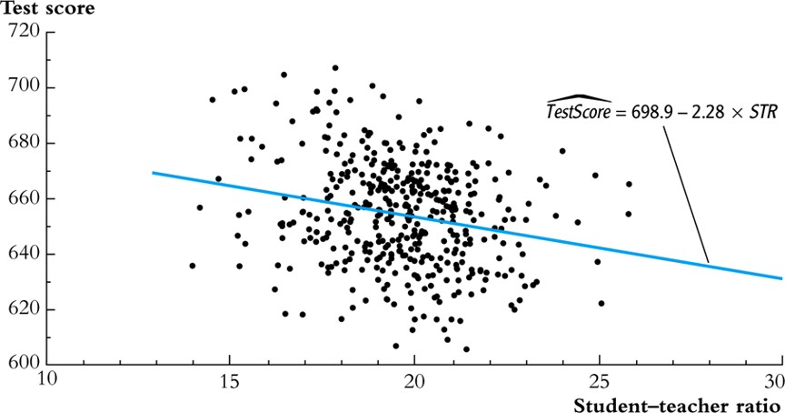
\includegraphics[width=.9\linewidth]{images/nonlin0.png}
\end{center}
\end{frame}

\begin{frame}{A linear fit on a non-linear relationship}
\begin{center}
    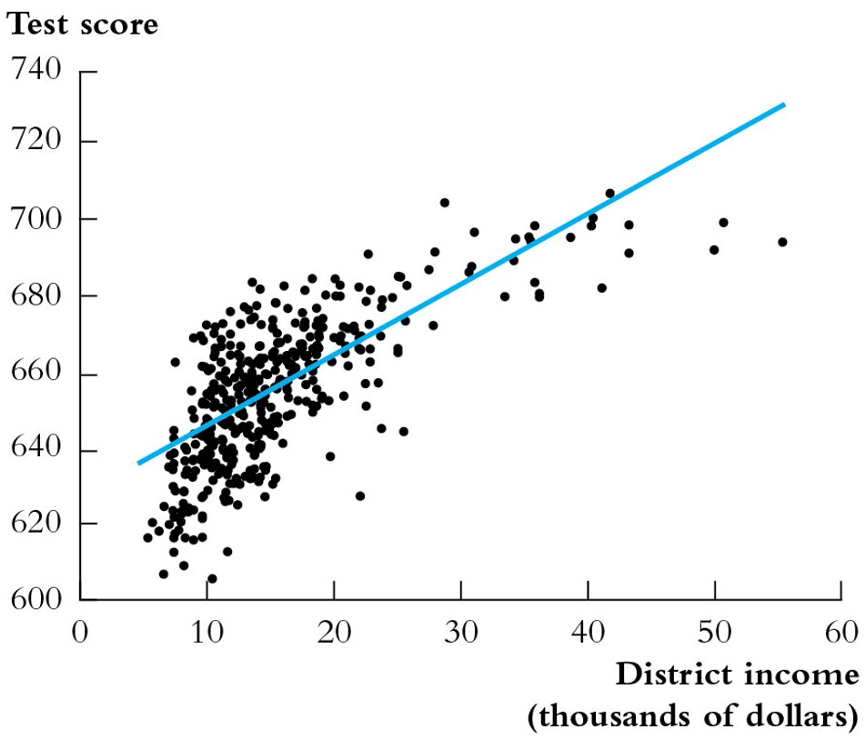
\includegraphics[width=.6\linewidth]{images/nonlin1.png}
\end{center}
\end{frame}



\begin{frame}{The general nonlinear population regression function}

The general nonlinear population regression function  is defined as
\begin{equation*}
    Y_i = f(X_{1i}, X_{2i}, \dots, X_{ki}) +u_i
\end{equation*}
Assumptions:
\begin{itemize}
    \item $\mathbb{E}(u_i\mid X_{1i}, X_{2i}, \dots, X_{ki})=0$ so $f(.)$ is the conditional expectation of $Y$ given the $X$'s.
    \item $(Y_i, X_{1i}, X_{2i}, \dots, X_{ki})$ are i.i.d.
    \item Big outliers are rare (same idea as with linear OLS; the precise mathematical condition depends on the specific $f(.)$).
    \item No perfect multicollinearity (same idea; the precise statement depends on the specific $f(.)$).
\end{itemize}

The expected difference in $Y$ associated with a difference in $X_1$, ceteris paribus, is

\begin{equation*}
    \Delta Y = f(X_{1} + \Delta X_{1}, X_{2}, \dots, X_{k}) -  f(X_{1}, X_{2}, \dots, X_{k}) 
\end{equation*}

\end{frame}


\begin{frame}{Nonlinear Functions of a Single Independent Variable}
We’ll look at two complementary approaches:\\[1em]

\begin{itemize}
    \item \textbf{Polynomials in $X$}
    \begin{itemize}
        \item The population regression function is approximated by a quadratic, cubic, or higher-degree polynomial
    \end{itemize}
    \vspace{1em}
    \item \textbf{Logarithmic transformations}
    \begin{itemize}
        \item $Y$ and/or $X$ is transformed by taking its logarithm, which provides a ``percentages'' interpretation (i.e., elasticities and semi-elasticities) of the coefficients that makes sense in many applications
    \end{itemize}
\end{itemize}
\vspace{1em}
The choice of specification (functional form) should be guided by judgment (which interpretation makes the most sense in your application?), tests, and plotting predicted values
\end{frame}


\begin{frame}{Polynomials in $X$}
Approximate the population regression function by a polynomial:
\begin{equation*}
    Y_i = \beta_0 + \beta_1 X_i + \beta_2 X_i^2 + \beta_3 X_i^3 + \dots + \beta_r X_i^r + u_i
\end{equation*}
\begin{itemize}
    \item This is just the linear multiple regression model -- except that the regressors are powers of $X$!
    \item  Estimation, hypothesis testing, etc. proceeds as in the multiple regression model using OLS
    \item The coefficients are difficult to interpret, but the regression function itself is interpretable
\end{itemize}
\vspace{1em}

For example, let's estimate the following quadratic specification:
\begin{equation*}
    \text{TestScore}_i = \beta_0 + \beta_1 \text{Income}_i + \beta_2 \text{Income}_i^2  + u_i
\end{equation*}
\end{frame}

\begin{frame}{Polynomials in $X$}
\textbf{Dependent variable: TestScore}
\begin{center}
\renewcommand{\arraystretch}{1.2}
\begin{tabular}{lr}
\toprule
Regressor & Coefficient \\
\midrule
$\text{Income}$ & $3.850995$ \\
$\text{Income}^2$ & $-0.0423085$ \\
Intercept & $607.3017$ \\
\bottomrule
\end{tabular}

\medskip
$n=420$ \qquad $R^2=0.5562$ \qquad $\mathrm{SER}=12.724$
\end{center}
\small Income is district per capita income, measured in thousands of dollars.
\end{frame}


\begin{frame}{Polynomials in $X$}
 \begin{columns}
\begin{column}{0.45\textwidth}
    \begin{itemize}
    \item We can plot the predicted values...\\[1em]
    \item The predicted change in $TestScore$ for a change in income from \$5K per capita to \$6K per capita is :\\[0.5em]
    $(6\times3.85 - 6^2\times 0.042)-(5\times3.85 - 5^2\times 0.042)=3.4$
    \end{itemize}
    \begin{table}[]
\begin{tabular}{|c|c|}
\hline
\rowcolor[HTML]{EFEFEF} 
\textbf{$\Delta Income$} & \textbf{$\Delta TestScore$} \\ \hline
from 5 to 6                             & 3.4                                        \\ \hline
from 25 to 26                           & 1.7                                        \\ \hline
from 45 to 46                           & 0.0                                          \\ \hline
\end{tabular}
\end{table}
    \begin{itemize}
    \item Caution! What is the effect of a change from \$100K to \$101K?  
    \end{itemize}

\end{column}
\begin{column}{0.6\textwidth}
\begin{figure}
  \centering
         \vspace{-2mm}
        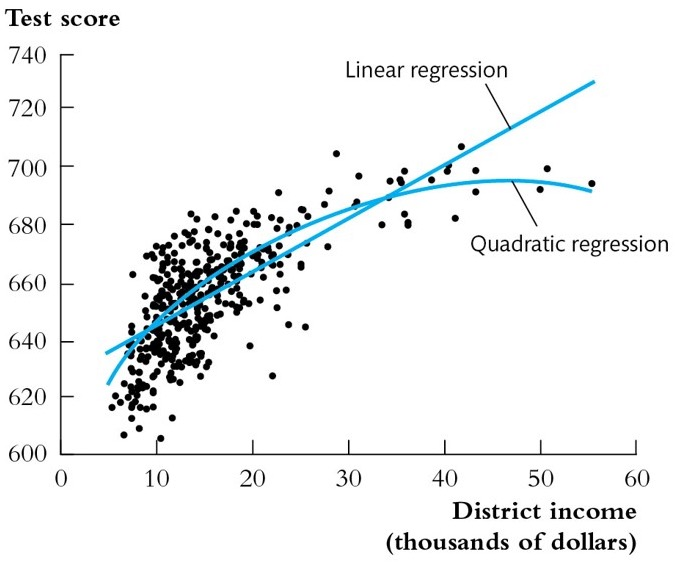
\includegraphics[scale=.3]{images/quadratic1.jpg}
\end{figure}
    \begin{itemize}
    \item The ``effect'' of a change in income is greater at low than high income levels (i.e., a declining marginal effect of income)
    \end{itemize}
\end{column}
\end{columns}
\end{frame}


\begin{frame}{Polynomials in $X$}
\textbf{Dependent variable: TestScore}
\begin{center}
\renewcommand{\arraystretch}{1.2}
\begin{tabular}{lr}
\toprule
Regressor & Coefficient \\
\midrule
$\text{Income}$ & $5.018677$ \\
$\text{Income}^2$ & $-0.0958052$ \\
$\text{Income}^3$ & $0.0006855$ \\
Intercept & $600.079$ \\
\bottomrule
\end{tabular}

\medskip
$n=420$ \qquad $R^2=0.5584$ \qquad $\mathrm{SER}=12.707$
\end{center}
\small Income is district per capita income, measured in thousands of dollars.
\end{frame}


\begin{frame}{Polynomials in $X$}
\small
\textbf{Link to Lecture 6: restricted versus unrestricted regression.}
\[
H_0:\beta_2=\beta_3=0
\qquad\text{vs.}\qquad
H_1:\beta_2\neq0\ \text{and/or}\ \beta_3\neq0.
\]
\textbf{Unrestricted ($U$):} estimate all four coefficients in the cubic model:
\[
\text{TestScore}_i=\beta_0+\beta_1\text{Income}_i
+\beta_2\text{Income}_i^2+\beta_3\text{Income}_i^3+u_i.
\]
\textbf{Restricted ($R$):} impose $H_0$ and re-estimate the linear model:
\[
\text{TestScore}_i=\beta_0+\beta_1\text{Income}_i+u_i.
\]
Thus $SSR_R=SSR_{\mathrm{linear}}$ and $SSR_U=SSR_{\mathrm{cubic}}$, using the same observations.
\[
\underbrace{F=\frac{(SSR_R-SSR_U)/q}{SSR_U/(n-k_U-1)}}_{\text{Lecture 6}}
=\frac{(SSR_{\mathrm{linear}}-SSR_{\mathrm{cubic}})/2}{SSR_{\mathrm{cubic}}/(n-4)}.
\]
$q=2$ restrictions; $k_U=3$ regressors (excluding the intercept), so $n-k_U-1=n-4$.
\medskip

Reject $H_0$ at 1\% if $F$ exceeds the $F_{2,n-4}$ critical value, or if $p<0.01$.
\end{frame}


\begin{frame}{Log Changes: Why the Approximation Works}
\small
Throughout these slides, $\log$ denotes the natural logarithm; $Y>0$.
\begin{columns}[T]
\begin{column}{0.52\textwidth}
\textbf{1. Approximate $\log(x)$ near $x=1$.}
\[
f(x)\approx f(1)+f'(1)(x-1).
\]
For $f(x)=\log(x)$, $f(1)=0$ and $f'(1)=1$, so
\[
\boxed{\log(x)\approx x-1\quad\text{near }x=1.}
\]
\textbf{2. Let $x$ be the ratio of new to old $Y$:}
\[
x=\frac{Y+\Delta Y}{Y}=1+\frac{\Delta Y}{Y}.
\]
A small proportional change makes $x$ close to 1.
\end{column}
\begin{column}{0.46\textwidth}
\centering
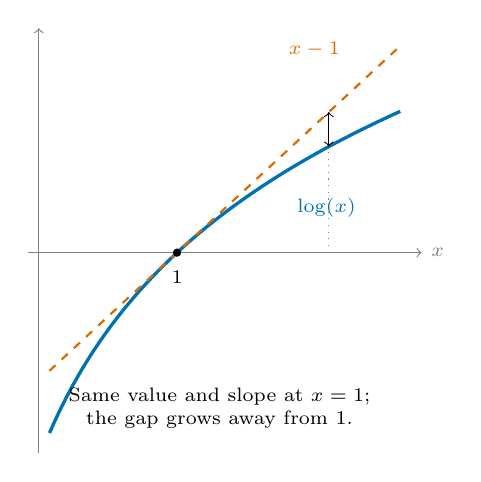
\begin{tikzpicture}[x=2.7cm,y=2.5cm,font=\scriptsize]
\draw[->,gray] (0.3,0)--(2.15,0) node[right] {$x$};
\draw[->,gray] (0.35,-1.02)--(0.35,1.14);
\draw[blue,very thick,domain=0.4:2.05,samples=90] plot (\x,{ln(\x)});
\draw[orange!85!black,thick,dashed,domain=0.4:2.05] plot (\x,{\x-1});
\fill (1,0) circle (1.5pt) node[below=3pt] {$1$};
\draw[gray,dotted] (1.714,0)--(1.714,0.714);
\draw[black,<->] (1.714,0.539)--(1.714,0.714);
\node[blue,anchor=west] at (1.52,0.23) {$\log(x)$};
\node[orange!85!black,anchor=west] at (1.48,1.03) {$x-1$};
\node[align=center] at (1.2,-0.79) {Same value and slope at $x=1$;\\the gap grows away from 1.};
\end{tikzpicture}
\end{column}
\end{columns}
\medskip
\textbf{3. Use the log-ratio identity and multiply by 100:}
\[
\log(Y+\Delta Y)-\log(Y)=\log\!\left(1+\frac{\Delta Y}{Y}\right)
\approx\frac{\Delta Y}{Y}
\quad\Rightarrow\quad
100\,\Delta\log Y\approx\text{percentage change in }Y.
\]
\end{frame}

\begin{frame}{Log Changes versus Percentage Changes}
\small
\textbf{Define two different measures of the same change:}
\[
g=\frac{Y_{\mathrm{new}}-Y_{\mathrm{old}}}{Y_{\mathrm{old}}},
\qquad d=\log(Y_{\mathrm{new}})-\log(Y_{\mathrm{old}})=\log(1+g).
\]
$100g$ is the percentage change; $100d$ is the change in \textbf{log points}.
\[
\boxed{g=e^d-1\quad\text{(exact)}}\qquad
\boxed{g\approx d\quad\text{(only for small changes)}}.
\]
\begin{center}
\begin{tabular}{lrr}
\toprule
Change in $Y$ & Actual change: $100g$ & Log points: $100\log(1+g)$\\
\midrule
$100\to101$ & $1.00\%$ & $1.00$\\
$100\to105$ & $5.00\%$ & $4.88$\\
$0.7\to1.2$ & $71.43\%$ & $53.90$\\
\bottomrule
\end{tabular}
\end{center}
\textbf{Our example is a large change:}
\[
g=\frac{1.2-0.7}{0.7}=0.7143,
\qquad d=\log(1.2/0.7)=0.5390\approx0.54.
\]
Thus about 54 log points correspond to a \textbf{71.4\% increase}, not a 54\% increase.\\
The approximation understates the increase by about 17.5 percentage points here.
\end{frame}

\begin{frame}{Why About 54 Successive Increases of 1\%?}
\small
\textbf{1. Each 1\% increase multiplies the current value by $1.01$.}
After $m$ such increases, $Y_{\mathrm{new}}=Y_{\mathrm{old}}(1.01)^m$.
\[
\log(Y_{\mathrm{new}}/Y_{\mathrm{old}})=m\log(1.01)
\quad\Rightarrow\quad
m=\frac{\log(1.2/0.7)}{\log(1.01)}
=\frac{0.5390}{0.009950}\approx54.17.
\]
\textbf{2. This explains the number 54:} each 1\% step adds about $0.01$ to the log.
\[
0.7(1.01)^{54}\approx1.198\approx1.2,
\qquad 100\big[(1.01)^{54}-1\big]\approx71.14\%.
\]
The increases compound: later 1\% increases apply to a larger base. Simply adding
$54\times1\%=54\%$ misses this growth of the base.
\medskip

\textbf{3. More generally, logarithms turn compounded growth into a sum.}
If $R_t=(Y_t-Y_{t-1})/Y_{t-1}$ is the proportional growth rate in period $t$,
\[
\frac{Y_T}{Y_0}=\prod_{t=1}^{T}(1+R_t)
\quad\Rightarrow\quad
\log(Y_T)-\log(Y_0)=\sum_{t=1}^{T}\log(1+R_t).
\]
This equality is exact. For small period-by-period changes, $\log(1+R_t)\approx R_t$.
\end{frame}


\begin{frame}{Logarithmic functions of $Y$ and/or $X$}
In the linear regression model,
\begin{eqnarray*}
    &Y_i &= \beta_0 + \beta_1 X_{1i} + u_i\\
\end{eqnarray*}
1-unit increase in $X_{1i}$ was associated with a $\beta_1$-unit increase in $Y_i$.\\[1em] 

Now, depending on the hypothesis we derived from the theory, data can be log-transformed on the RHS or the LHS or both.\\

\begin{eqnarray*}
    &Y_i &= \beta_0 + \beta_1 log(X_{1i}) + u_i\\
    &log(Y_i) &= \beta_0 + \beta_1 X_{1i} + u_i\\
    &log(Y_i) &= \beta_0 + \beta_1 log(X_{1i}) + u_i\\
\end{eqnarray*}
In each case, $\beta_1$ has a different interpretation.
\end{frame}


\begin{frame}{Linear-log: Rising but Flattening}
\small
\setlength{\abovedisplayskip}{4pt}
\setlength{\belowdisplayskip}{4pt}
\setlength{\abovedisplayshortskip}{2pt}
\setlength{\belowdisplayshortskip}{2pt}
\begin{columns}[T]
\begin{column}{0.56\textwidth}
\textbf{Model and change (holding $u$ fixed):}
\[
Y=\beta_0+\beta_1\log X+u,
\]
\[
\Delta Y=\beta_1[\log(X+\Delta X)-\log X]
\approx\beta_1\frac{\Delta X}{X}.
\]
\textbf{A 1\% increase in $X$:}
\[
\frac{\Delta X}{X}=0.01
\quad\Rightarrow\quad
\Delta Y\approx\frac{\beta_1}{100}.
\]
This is a change in \textbf{units of $Y$}, not percent. With $\beta_1=20$, it is about $0.2$ units.
\vspace{3pt}

\textbf{Why does the curve flatten?}
\[
\boxed{\frac{dY}{dX}=\frac{\beta_1}{X}.}
\]
For $\beta_1>0$, a larger $X$ means a smaller slope: the same extra unit of $X$ adds less to $Y$.
\end{column}
\begin{column}{0.41\textwidth}
\centering
\textbf{Example: $Y=20\log X$}

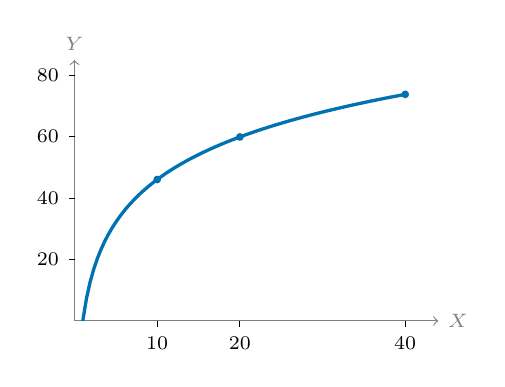
\begin{tikzpicture}[x=0.105cm,y=0.039cm,font=\scriptsize]
\draw[->,gray] (0,0)--(44,0) node[right] {$X$};
\draw[->,gray] (0,0)--(0,85) node[above] {$Y$};
\draw[blue,very thick,domain=1:40,samples=90] plot (\x,{20*ln(\x)});
\foreach \x in {10,20,40} {
\draw (\x,0)--(\x,-2) node[below] {\x};
\fill[blue] (\x,{20*ln(\x)}) circle(1.4pt);
}
\foreach \y in {20,40,60,80} \draw (0,\y)--(-0.7,\y) node[left] {\y};
\end{tikzpicture}

\vspace{3pt}
\begin{tabular}{c|ccc}
$X$ & 10 & 20 & 40\\
\hline
Slope $20/X$ & 2 & 1 & 0.5
\end{tabular}
\vspace{3pt}

\raggedright
Doubling $X$ always adds $20\log 2\approx13.86$ units to $Y$, but requires a larger dollar increase at higher $X$.
\end{column}
\end{columns}
\vspace{3pt}
{\scriptsize Graphs use the original $X,Y$ axes and set $u=0$. With $\beta_1<0$, this curve decreases and becomes less steep.}
\end{frame}

\begin{frame}{Log-linear: Constant Percentage Growth}
\small
\setlength{\abovedisplayskip}{4pt}
\setlength{\belowdisplayskip}{4pt}
\setlength{\abovedisplayshortskip}{2pt}
\setlength{\belowdisplayshortskip}{2pt}
\begin{columns}[T]
\begin{column}{0.56\textwidth}
\textbf{Model and change (holding $u$ fixed):}
\[
\log Y=\beta_0+\beta_1X+u,
\qquad \Delta\log Y=\beta_1\Delta X.
\]
For a small log change, $\Delta\log Y\approx\Delta Y/Y$.
\vspace{3pt}

\textbf{A one-unit increase in $X$:}
\[
\Delta X=1
\ \Rightarrow\ \frac{\Delta Y}{Y}\approx\beta_1
\ \Rightarrow\ 100\frac{\Delta Y}{Y}\approx100\beta_1.
\]
Multiplying by 100 gives the \textbf{percentage change in $Y$}.
\vspace{3pt}

With $\beta_1=0.05$, one extra unit of $X$ gives about 5\% more $Y$, not 5 units.
\[
\text{Exact change}=100(e^{0.05}-1)\%\approx5.13\%.
\]
\textbf{Why does the curve steepen?}
\[
Y=e^{\beta_0+\beta_1X}\ (u=0),
\qquad\boxed{\frac{dY}{dX}=\beta_1Y.}
\]
For $\beta_1>0$, the same percentage increase applies to a growing base: the gain in units gets larger.
\end{column}
\begin{column}{0.41\textwidth}
\centering
\textbf{Example: $Y=10e^{0.05X}$}

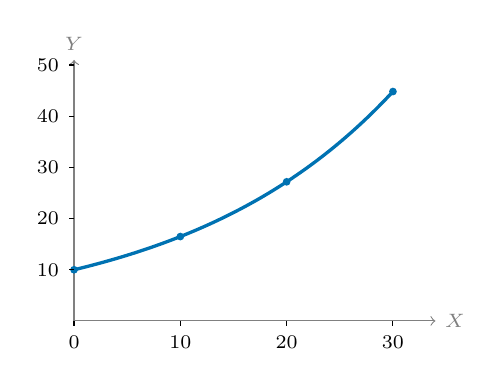
\begin{tikzpicture}[x=0.135cm,y=0.065cm,font=\scriptsize]
\draw[->,gray] (0,0)--(34,0) node[right] {$X$};
\draw[->,gray] (0,0)--(0,51) node[above] {$Y$};
\draw[blue,very thick,domain=0:30,samples=90] plot (\x,{10*exp(0.05*\x)});
\foreach \x in {0,10,20,30} {
\draw (\x,0)--(\x,-1) node[below] {\x};
\fill[blue] (\x,{10*exp(0.05*\x)}) circle(1.4pt);
}
\foreach \y in {10,20,30,40,50} \draw (0,\y)--(-0.5,\y) node[left] {\y};
\end{tikzpicture}

\vspace{3pt}
\begin{tabular}{c|ccc}
$X$ & 0 & 10 & 20\\
\hline
$Y$ & 10 & 16.49 & 27.18\\
Slope $0.05Y$ & 0.50 & 0.82 & 1.36
\end{tabular}
\vspace{3pt}

\raggedright
The curve is exponential on $X,Y$ axes. It becomes a \textbf{straight line} on $X,\log Y$ axes (as in slide 21).
\end{column}
\end{columns}
\vspace{3pt}
{\scriptsize The graph sets $u=0$. For $\beta_1<0$, exponential decay approaches zero and becomes less steep.}
\end{frame}

\begin{frame}{Log-log: The Elasticity Determines the Shape}
\small
\setlength{\abovedisplayskip}{4pt}
\setlength{\belowdisplayskip}{4pt}
\setlength{\abovedisplayshortskip}{2pt}
\setlength{\belowdisplayshortskip}{2pt}
\begin{columns}[T]
\begin{column}{0.56\textwidth}
\textbf{Model and change (holding $u$ fixed):}
\[
\log Y=\beta_0+\beta_1\log X+u,
\]
\[
\Delta\log Y=\beta_1\Delta\log X
\quad\Rightarrow\quad
\frac{\Delta Y}{Y}\approx\beta_1\frac{\Delta X}{X}.
\]
\textbf{A 1\% increase in $X$:}
\[
\frac{\Delta X}{X}=0.01
\quad\Rightarrow\quad
100\frac{\Delta Y}{Y}\approx\beta_1.
\]
So $Y$ changes by approximately $\beta_1$\%. Here $\beta_1$ is the \textbf{elasticity}.
\vspace{3pt}

\textbf{Shape in levels:} with $A=e^{\beta_0}>0$ and $u=0$,
\[
Y=AX^{\beta_1},
\qquad\boxed{\frac{dY}{dX}=A\beta_1X^{\beta_1-1}.}
\]
\begin{itemize}\setlength{\itemsep}{1pt}
\item $0<\beta_1<1$: rises and flattens.
\item $\beta_1=1$: straight line through the origin.
\item $\beta_1>1$: rises and steepens.
\end{itemize}
\end{column}
\begin{column}{0.41\textwidth}
\centering
\textbf{Examples with $A=1$: $Y=X^{\beta_1}$}

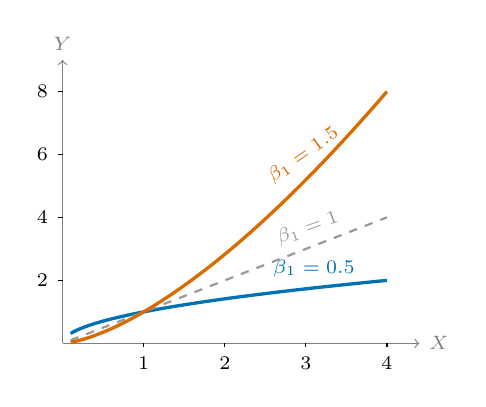
\begin{tikzpicture}[x=1.03cm,y=0.4cm,font=\scriptsize]
\draw[->,gray] (0,0)--(4.4,0) node[right] {$X$};
\draw[->,gray] (0,0)--(0,9) node[above] {$Y$};
\draw[blue,very thick,domain=0.1:4,samples=90] plot (\x,{sqrt(\x)});
\draw[gray!80,thick,dashed] (0.1,0.1)--(4,4);
\draw[orange!85!black,very thick,domain=0.1:4,samples=90] plot (\x,{pow(\x,1.5)});
\foreach \x in {1,2,3,4} \draw (\x,0)--(\x,-0.12) node[below] {\x};
\foreach \y in {2,4,6,8} \draw (0,\y)--(-0.06,\y) node[left] {\y};
\node[blue,above] at (3.1,1.8) {$\beta_1=0.5$};
\node[gray!80,above,rotate=20] at (3.1,3.1) {$\beta_1=1$};
\node[orange!85!black,above,rotate=35] at (3.1,5.5) {$\beta_1=1.5$};
\end{tikzpicture}

\vspace{3pt}
\raggedright
For $\beta_1=0.5$, a 1\% increase in $X$ gives about 0.5\% more $Y$; for $\beta_1=1.5$, about 1.5\% more $Y$.
\vspace{3pt}

All three become straight lines on \textbf{$\log X,\log Y$ axes}, with slopes $\beta_1$.
\end{column}
\end{columns}
\vspace{3pt}
{\scriptsize Graphs use the original $X,Y$ axes. If $\beta_1<0$, $Y$ decreases and flattens; if $\beta_1=0$, it is constant.}
\end{frame}

\begin{frame}{(Linear-)Cubic vs. Linear-Log}
\begin{center}
    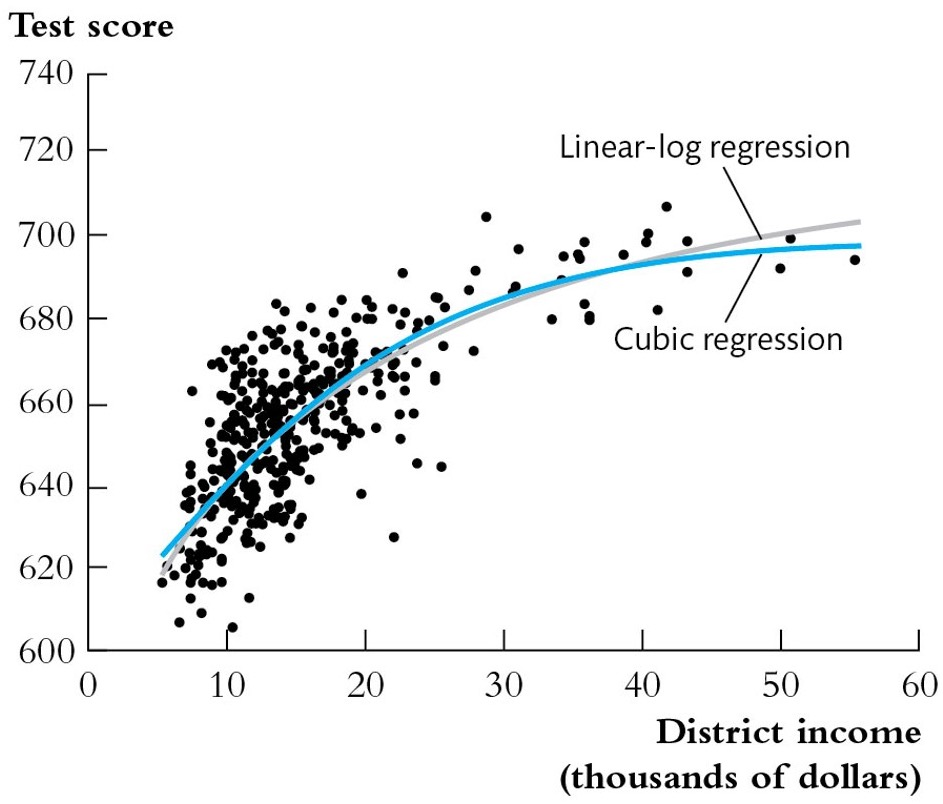
\includegraphics[width=.6\linewidth]{images/linlog.jpg}
\end{center}
\end{frame}



\begin{frame}{Log-Linear vs. Log-Log}
\begin{center}
    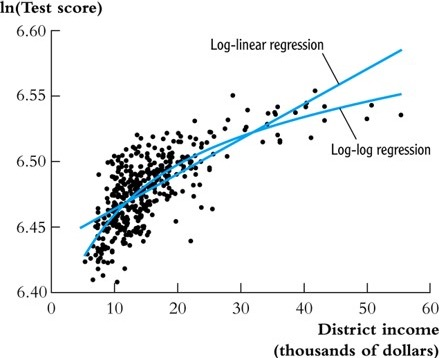
\includegraphics[width=.6\linewidth]{images/loglog.jpg}
\end{center}
\end{frame}


\begin{frame}{Interactions and heterogenous effects}
\begin{itemize}
    \item In the California Schools example, at the beginning of the course, we were interested in knowing the impact of the Share of Subsidized Meals on TestScores\\[1em]
    \item We saw that the Share of Subsidized Meals was, on average, negatively associated with TestScores\\[1em]
    \item We said that the impact of the Share of Subsidized Meals on on TestScores could be cofounded by local Educational Attainment\\[1em]
    \item But we might be interested in knowing the \textit{heterogenous} effects of the Share of Subsidized Meals depending on different levels of Educational Attainment\\[1em]
    \item Is the effect of subsidizing meals still associated with lower test scores, even when local educational attainment is low?
\end{itemize}
\end{frame}

\begin{comment}
\begin{frame}{Interactions between two dummies}
Consider the following specification
\begin{equation*}
    Y_i = \beta_0 + \beta_1 D_{1i} + \beta_2 D_{2i} + \beta_3 (D_{1i} \times D_{2i}) + u_i
\end{equation*}
where $D_{1i}$ and $D_{2i}$ are dummy variables.\\[1em]
\begin{itemize}
    \item $\beta_1$ is the unconditional effect of $D_{1}$ alone, i.e., irrespective of the value of $D_{2}$
    \item $\beta_2$ is the unconditional effect of $D_{2}$ alone, i.e., irrespective of the value of  $D_{1}$
    \item $\beta_3$ is the \textit{interaction} effect of $D_{1}=1$ and $D_{2}=1$, i.e., the additional effect of an increase in both $D_{1}$ and $D_{2}$, at the same time
\end{itemize}
\end{frame}
\end{comment}

\begin{frame}{Interactions between two dummies}
Consider the following specification
\begin{equation*}
    Y_i = \beta_0 + \beta_1 D_{1i} + \beta_2 D_{2i} + \beta_3 (D_{1i} \times D_{2i}) + u_i
\end{equation*}
where $D_{1i}$ and $D_{2i}$ are dummy variables.\\[1em]
\begin{itemize}
    \item (Comparison category) $D_{1i}=0$ and $D_{2i}=0$ $\Rightarrow \mathbb{E}(Y\mid D_{1i}=0, D_{2i}=0) = \beta_0$ 
    \item When $D_{1i}=1$ but $D_{2i}=0$ $\Rightarrow \mathbb{E}(Y\mid D_{1i}=1, D_{2i}=0) = \beta_0 + \beta_1$ 
    \item When $D_{1i}=0$ but $D_{2i}=1$ $\Rightarrow \mathbb{E}(Y\mid D_{1i}=0, D_{2i}=1) = \beta_0 + \beta_2$ 
    \item Full model when $D_{1i}=1$ and $D_{2i}=1$ $\Rightarrow \mathbb{E}(Y\mid D_{1i}=1, D_{2i}=1) = \beta_0 + \beta_1 + \beta_2 + \beta_3$ 
\end{itemize}
\vspace{1em}
$\beta_3$ can be interpreted as the incremental effect to $D_{1}$ (resp. $D_{2}$) \underline{when} $D_{2}=1$ (resp. $D_{1}=1$)
\end{frame}

\begin{frame}{Interactions between two dummies}
\textbf{Dependent variable: TestScore}
\begin{center}
\renewcommand{\arraystretch}{1.2}
\begin{tabular}{lr}
\toprule
Regressor & Coefficient \\
\midrule
$H$ & $-62.37116$ \\
$L$ & $-42.54073$ \\
$H \times L$ & $24.82402$ \\
Intercept & $796.65$ \\
\bottomrule
\end{tabular}

\medskip
$n=500$ \qquad $R^2=0.3605$ \qquad $\mathrm{SER}=48.368$
\end{center}
\small $H=\texttt{high\_share\_meals}$ indicates the high subsidized-meal-share group; $L=\texttt{low\_educ}$ indicates the low educational-attainment group. Each dummy is 1 for its named group and 0 otherwise.
\end{frame}



\begin{frame}{Interactions between a dummy and a continuous variable}
How to think about dummies in the presence of a continuous variables? First, consider the simple case without interaction:
\begin{equation*}
    Y_i = \beta_0 + \beta_1 X_{1i} + \beta_2 D_{1i} 
 + u_i
\end{equation*}
where $D_{1i}$ is a dummy and $X_{1i}$ is a continuous variable.\\[1em]

The regression line when $D_1=0$ reads
\begin{equation*}
    \mathbb{E}(Y\mid D_{1i}=0, X_{1i}) = \beta_0 +  \beta_1 X_{2i} 
\end{equation*}
While the regression line when $D_1=1$ reads
\begin{equation*}
    \mathbb{E}(Y\mid D_{1i}=1, X_{1i}) = (\beta_0 + \beta_2) + \beta_1 X_{1i} 
\end{equation*}
The intercepts are different but the slopes are the same!
\end{frame}

\begin{frame}{Interactions between a dummy and a continuous variable}
\begin{center}
    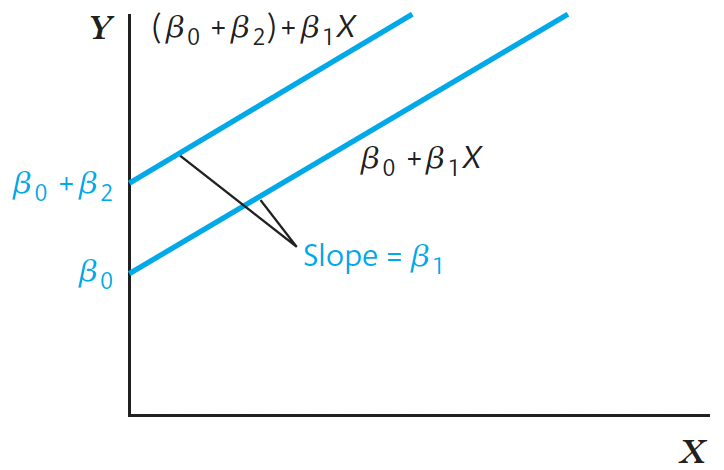
\includegraphics[width=.75\linewidth]{images/inter1.png}
\end{center}
\end{frame}



\begin{frame}{Interactions between a dummy and a continuous variable}
This framework can be extended to the interaction between a dummy and a continuous variable. Next, consider
\begin{equation*}
    Y_i = \beta_0 + \beta_1 X_{1i} + \beta_2 (D_{1i} \times X_{1i}) + u_i
\end{equation*}
where $D_{1i}$ is a dummy and $X_{1i}$ is a continuous variable.\\[1em]

The regression line when $D_1=0$ reads
\begin{equation*}
    \mathbb{E}(Y\mid D_{1i}=0, X_{1i}) = \beta_0 +  \beta_1 X_{1i} 
\end{equation*}
While the regression line when $D_1=1$ reads
\begin{equation*}
    \mathbb{E}(Y\mid D_{1i}=1, X_{1i}) = \beta_0 + \ (\beta_1 + \beta_2) X_{1i} 
\end{equation*}
The intercept is the same, but slopes are different!
\end{frame}

\begin{frame}{Interactions between a dummy and a continuous variable}
\begin{center}
    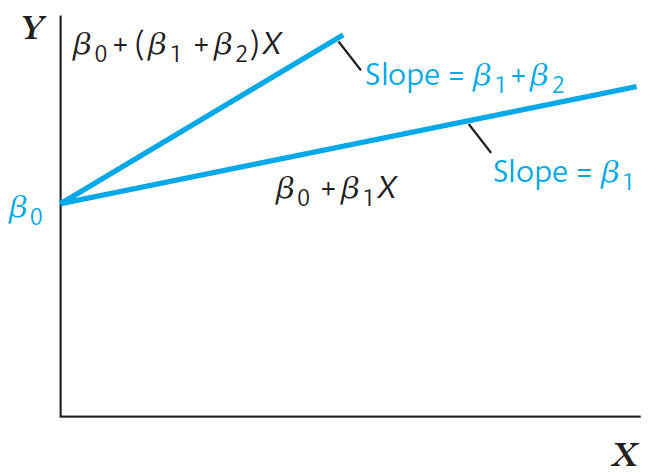
\includegraphics[width=.7\linewidth]{images/inter2.png}
\end{center}
\end{frame}


\begin{frame}{Interactions between a dummy and a continuous variable}
Next consider the fully interacted model:
\begin{equation*}
    Y_i = \beta_0 + \beta_1 D_{1i} + \beta_2 X_{1i} + \beta_3 (D_{1i} \times X_{1i}) + u_i
\end{equation*}
where $D_{1i}$ is a dummy and $X_{1i}$ is a continuous variable.\\[1em]

The regression line when $D_1=0$ reads
\begin{equation*}
    \mathbb{E}(Y\mid D_{1i}=0, X_{1i}) = \beta_0 +  \beta_2 X_{1i} 
\end{equation*}
While the regression line when $D_1=1$ reads
\begin{equation*}
    \mathbb{E}(Y\mid D_{1i}=1, X_{1i}) = (\beta_0 + \beta_1) + (\beta_2 + \beta_3) X_{1i} 
\end{equation*}
The intercepts and slopes depend on the groups defined by $D_1$!
\end{frame}

\begin{frame}{Interactions between a dummy and a continuous variable}
\begin{center}
    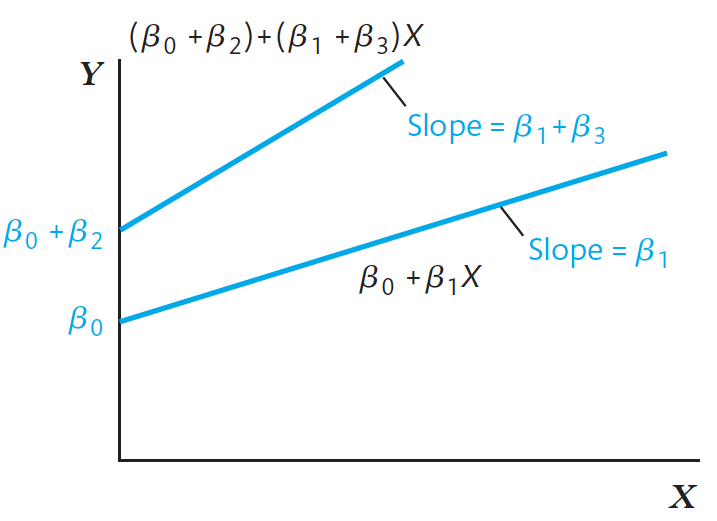
\includegraphics[width=.7\linewidth]{images/inter3.png}
\end{center}
\end{frame}


\begin{frame}{Interactions between a dummy and a continuous variable}
\textbf{How to discriminate between the last 3 models?}\\[1em]
Run the fully interacted model
\begin{equation*}
    Y_i = \beta_0 + \beta_1 D_{1i} + \beta_2 X_{1i} + \beta_3 (D_{1i} \times X_{1i}) + u_i
\end{equation*}
\begin{itemize}
    \item \textbf{Test if the two lines are the same ---} (In other words, does the interaction matter?) Compute the F-statistic testing the joint hypothesis that $\beta_1=\beta_3=0$ (Chow Test)\\[1em]
    \item \textbf{Test if the two lines have the same slope ---} Compute the t-statistic testing the simple hypothesis that $\beta_3=0$  \\[1em]
    \item \textbf{Test if the two lines have the same intercept ---} Compute the t-statistic testing the simple hypothesis that $\beta_1=0$ 
\end{itemize}
\end{frame}




\begin{frame}{Interactions between a dummy and a continuous variable}
\textbf{Dependent variable: TestScore}
\begin{center}
\renewcommand{\arraystretch}{1.2}
\begin{tabular}{lr}
\toprule
Regressor & Coefficient \\
\midrule
$S$ & $-162.5841$ \\
$L$ & $-46.65102$ \\
$S \times L$ & $56.57384$ \\
Intercept & $853.1778$ \\
\bottomrule
\end{tabular}

\medskip
$n=500$ \qquad $R^2=0.5143$ \qquad $\mathrm{SER}=42.153$
\end{center}
\small $S=\texttt{frpm\_frac\_s}$ is the share of students eligible for free or reduced-price meals. $L=\texttt{low\_educ}$ is 1 for the low educational-attainment group and 0 otherwise.
\end{frame}


\begin{frame}{Interactions between a dummy and a continuous variable}
\begin{center}
    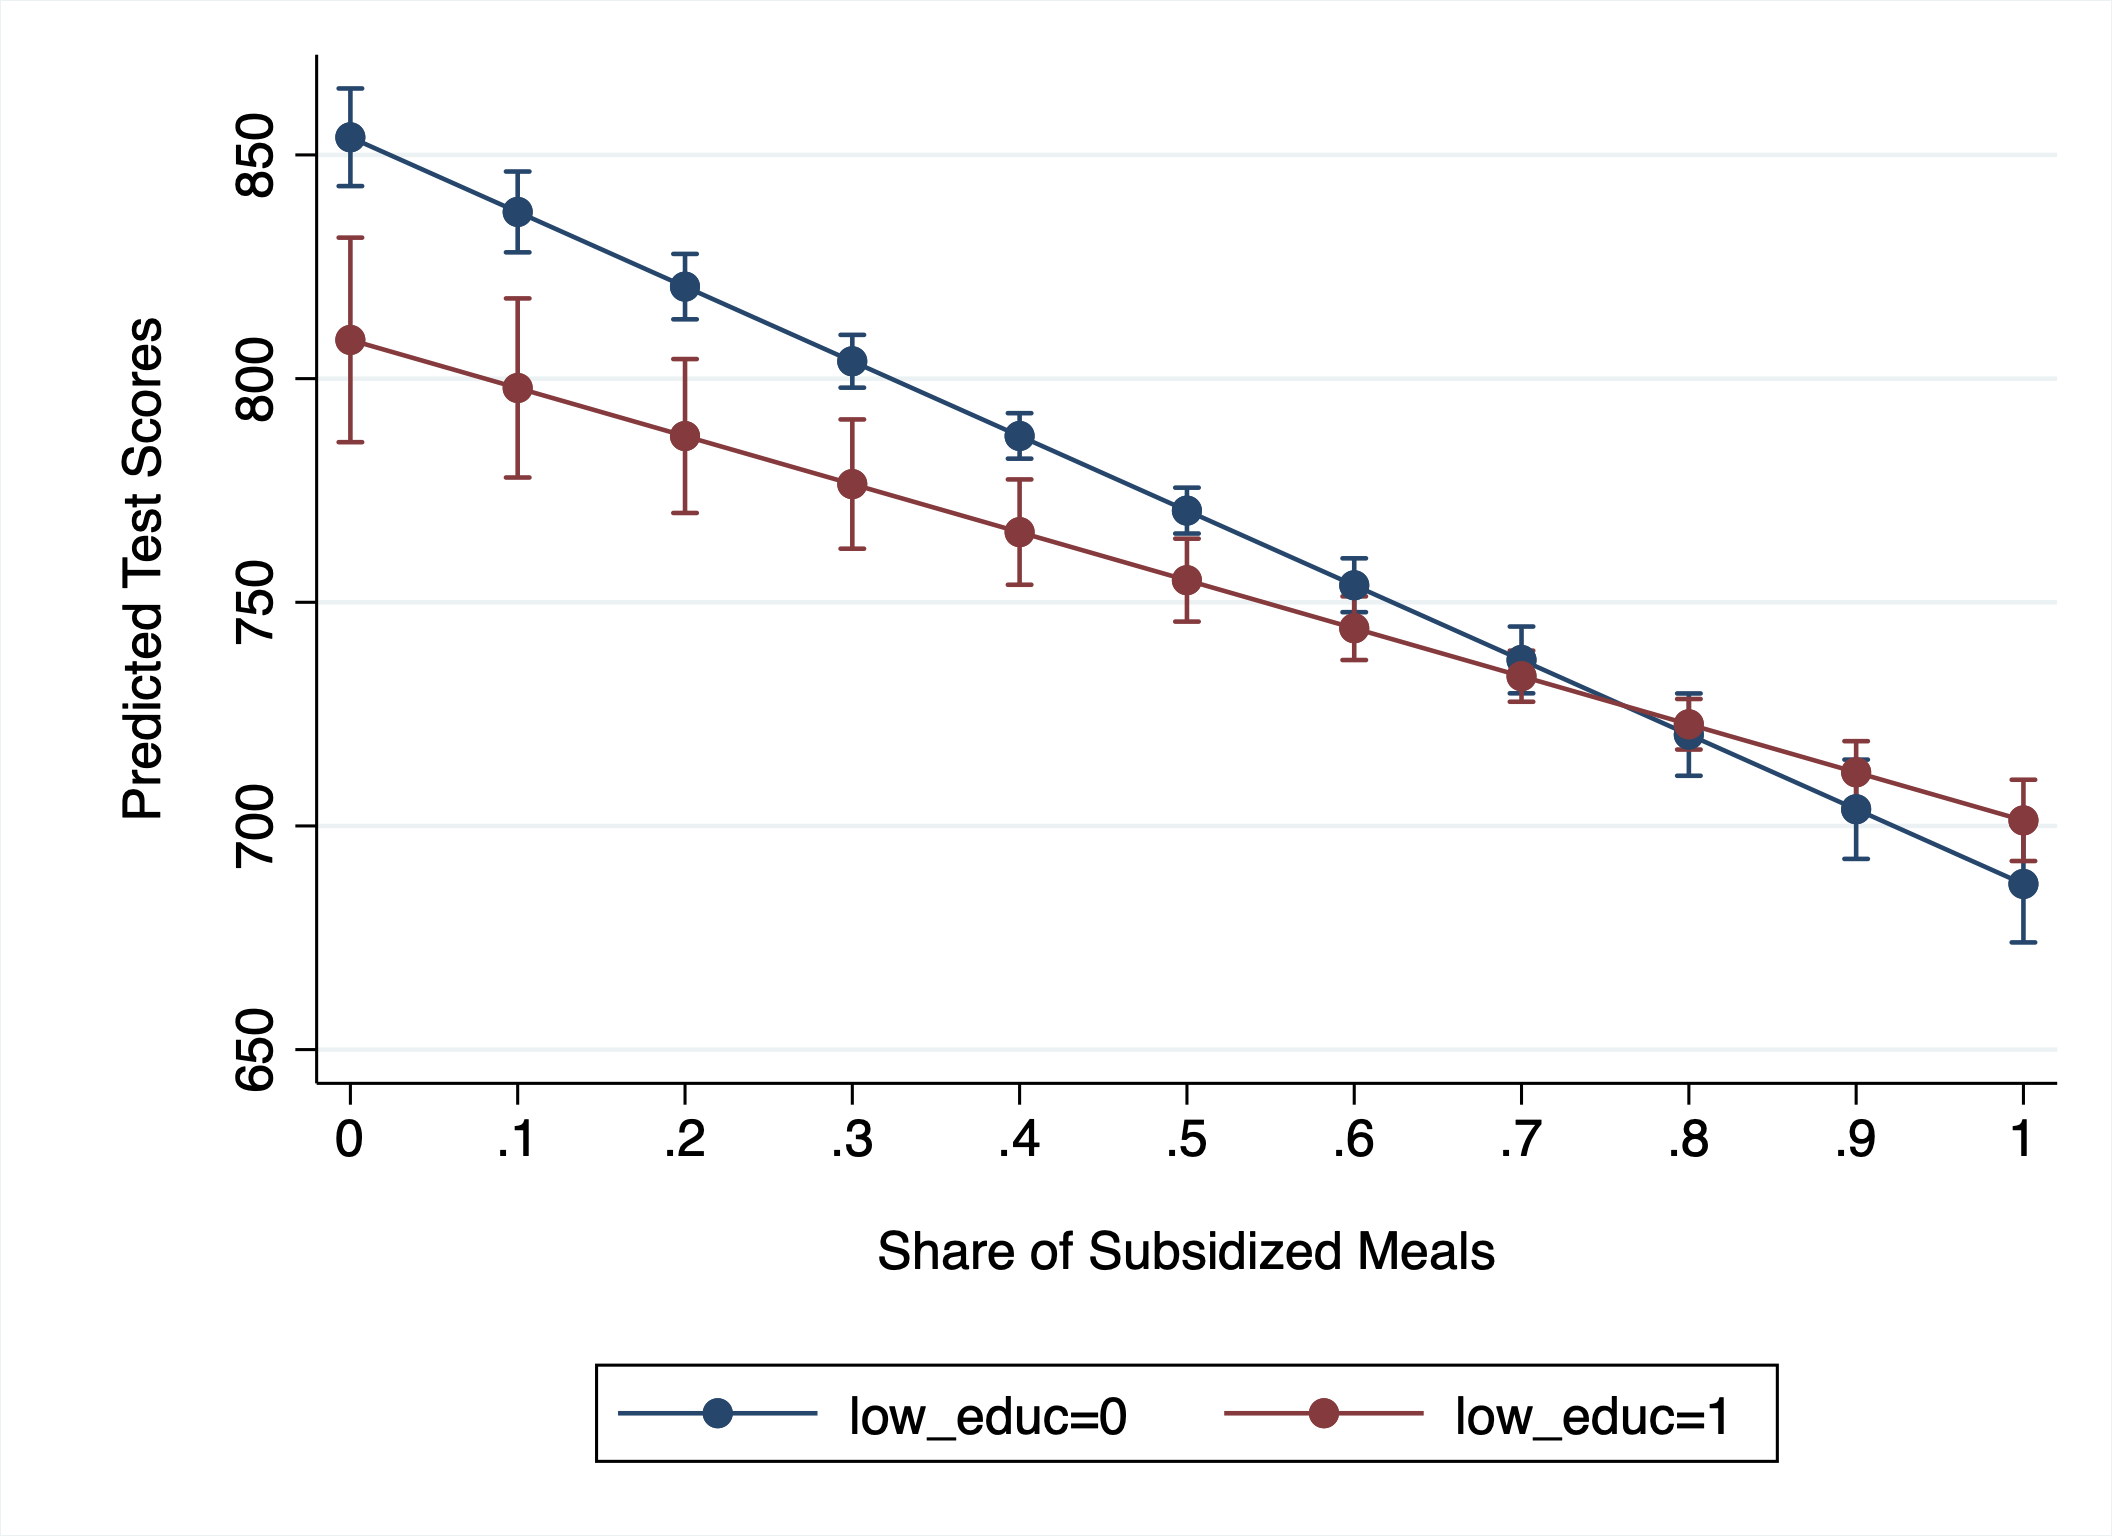
\includegraphics[width=.75\linewidth]{images/contdumgraph.png}
\end{center}
\end{frame}

\begin{comment}
\begin{frame}{Interactions between a dummy and a continuous variable}
This framework can be extended to the interaction between a dummy and a continuous variable
\begin{equation*}
    Y_i = \beta_0 + \beta_1 D_{1i} + \beta_2 X_{2i} + \beta_3 (D_{1i} \times X_{2i}) + u_i
\end{equation*}
where $D_{1i}$ is a dummy and $X_{2i}$ is a continuous variable.\\[1em]

The regression line when $D_1=0$ reads
\begin{equation*}
    \mathbb{E}(Y\mid D_{1i}=0, X_{2i}) = \beta_0 +  \beta_2 X_{2i} 
\end{equation*}
While the regression line when $D_1=1$ reads
\begin{equation*}
    \mathbb{E}(Y\mid D_{1i}=0, X_{2i}) = (\beta_0 + \beta_1) + (\beta_2 + \beta_3) X_{2i} 
\end{equation*}
The intercepts and slopes depend on $D_1$.
\end{frame}


\begin{frame}{Interactions between a dummy and a continuous variable}
\textbf{Dependent variable: TestScore}
\begin{center}
\renewcommand{\arraystretch}{1.2}
\begin{tabular}{lr}
\toprule
Regressor & Coefficient \\
\midrule
$S$ & $-162.5841$ \\
$L$ & $-46.65102$ \\
$S \times L$ & $56.57384$ \\
Intercept & $853.1778$ \\
\bottomrule
\end{tabular}

\medskip
$n=500$ \qquad $R^2=0.5143$ \qquad $\mathrm{SER}=42.153$
\end{center}
\small $S=\texttt{frpm\_frac\_s}$ is the share of students eligible for free or reduced-price meals. $L=\texttt{low\_educ}$ is 1 for the low educational-attainment group and 0 otherwise.
\end{frame}

\begin{frame}{Interactions between a dummy and a continuous variable}
\begin{center}
    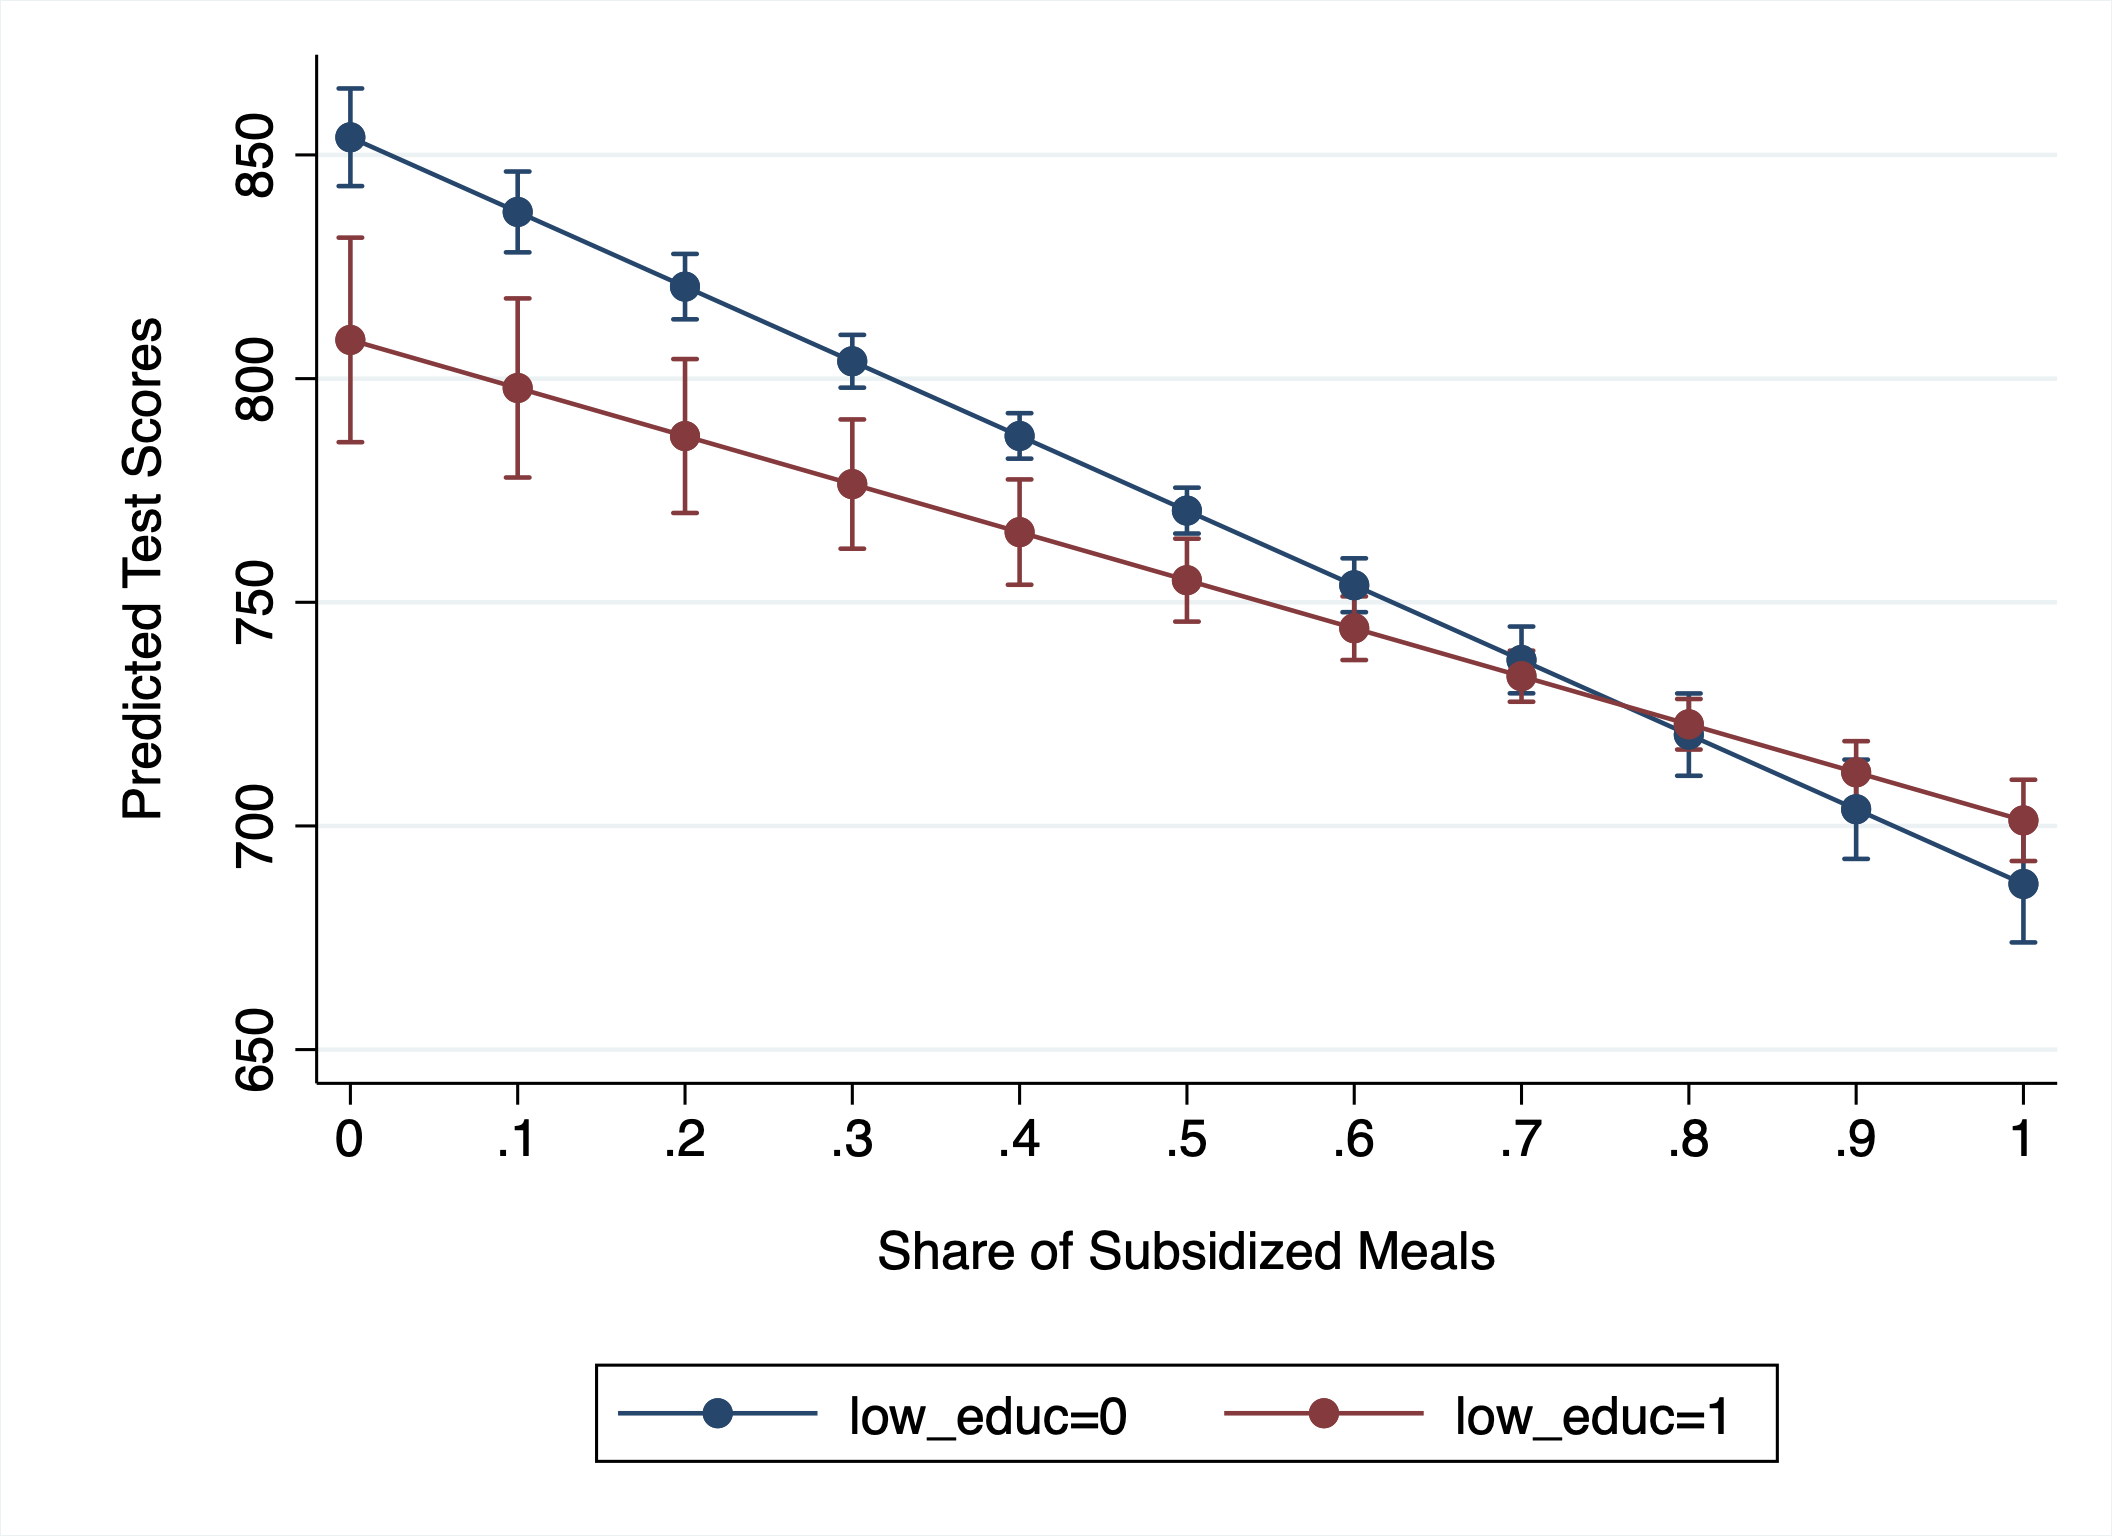
\includegraphics[width=.88\linewidth]{images/contdumgraph.png}
\end{center}
\end{frame}


\begin{frame}{Interactions between a dummy and a continuous variable}
We can extend this to two continuous variables
\begin{equation*}
    Y_i = \beta_0 + \beta_1 X_{1i} + \beta_2 X_{2i} + \beta_3 (X_{1i} \times X_{2i}) + u_i
\end{equation*}
where both $X_{1i}$ and $X_{2i}$ are continuous variable.\\[1em]

A change in $Y$ due to $X_1$ reads
\begin{equation*}
    Y_i + \Delta Y_i = \beta_0 + \beta_1 (X_{1i} + \Delta X_{1i} ) + \beta_2 X_{2i} + \beta_3 [(X_{1i} + \Delta X_{1i} ) \times X_{2i}] + u_i
\end{equation*}

Therefore,

\begin{equation*}
    \Delta Y_i = \beta_1\Delta X_{1i} + \beta_3 (\Delta X_{1i} \times X_{2i}) = \Delta X_{1i} (\beta_1 + \beta_3 X_{2i}) \text{~~~i.e.,~~}\frac{\Delta Y}{\Delta X_{1}} = \beta_1 + \beta_3 X_{2}
\end{equation*}
\\[1em]
We made obvious that the impact of $X_1$ on $Y$ varies with $X_2$!
\end{frame}


\end{comment}

\begin{frame}{Interactions between two continuous variable}
\textbf{Dependent variable: TestScore}
\begin{center}
\renewcommand{\arraystretch}{1.2}
\begin{tabular}{lr}
\toprule
Regressor & Coefficient \\
\midrule
$S$ & $-245.3094$ \\
$E$ & $-159.7155$ \\
$S \times E$ & $161.8956$ \\
Intercept & $944.4173$ \\
\bottomrule
\end{tabular}

\medskip
$n=500$ \qquad $R^2=0.5325$ \qquad $\mathrm{SER}=41.358$
\end{center}
\small $S=\texttt{frpm\_frac\_s}$ is the share of students eligible for free or reduced-price meals. $E$ is the education measure (\texttt{ed\_frac\_sc\_lesscollege}).
\end{frame}



\begin{frame}
\frametitle{Wrapping up: Linear vs. Non-Linear Models}

\textbf{In econometrics, we initially favor linear models for their simplicity:}
\begin{itemize}
    \item Linear models assume a constant relationship between variables (e.g., a one-unit increase in $X$ leads to a fixed change in $Y$).
    \item However, economic relationships are often complex and dynamic, and this assumption \textit{might not hold in reality}.
    \item Non-linear models, in contrast, allow for more flexible and \textit{realistic} relationships. They can capture intricate economic behaviors that linear models cannot.
\end{itemize}
\vspace{1em}
\textbf{In practice, numerous economic phenomena exhibit non-linear characteristics:}
\begin{itemize}
    \item For example, consider luxury goods. The demand for such goods may not increase linearly with income. As income rises, the demand might accelerate.
    \item Using linear models in such cases can lead to biased and inaccurate results because they fail to capture these \textit{nuanced relationships.}
    \item Recognizing non-linear patterns in data is essential for \textit{accurately} modeling and understanding real-world economic dynamics.
\end{itemize}

\end{frame}




\begin{frame}
\frametitle{The Importance of Interactions}

\textbf{Interactions in econometrics refer to how the effect of one variable depends on the level of another:}
\begin{itemize}
    \item Non-linear interactions can be critical in economic analysis. They enable us to explore \textit{how the relationship between two variables changes as one variable varies}.
    \item For instance, think about the interaction between interest rates and GDP. The impact of interest rates on investment may vary at different levels of GDP. In times of economic growth, a change in interest rates might have a stronger or weaker effect on investment.
    \item By incorporating non-linear interactions, we gain a more nuanced understanding of the \textit{interplay between variables}, making our models more realistic and insightful.
\end{itemize}
\vspace{1em}
$\longrightarrow$ Choosing the right functional form may not only improve your predictive power, it can also have large policy implications!
\end{frame}



\begin{frame}[allowframebreaks]{Material}
\begin{itemize}
    \item[--] \textbf{Textbooks:}
    \begin{itemize}
        \item Introduction to Econometrics, 4th Edition, Global Edition, by Stock and Watson -- Chapter 8.
    \end{itemize}
\end{itemize}
\end{frame}


\end{document}
